% fig_assignment: assignment interdiction on a toy instance.  The follower assigns 4 workers
% (rows) to 4 jobs (columns) at the least total cost; the leader first forbids 2 pairs
% (each ban costs 1, budget 2) to make that least cost as high as possible.
% Data (checked by brute force over all 120 pairs of bans and all 24 assignments):
%   costs  1 8 9 7 / 5 5 8 1 / 9 7 4 3 / 9 2 5 2   (row = worker, column = job).
%   No ban: cheapest assignment 1->1, 2->4, 3->3, 4->2, cost 1+1+4+2 = 8 (unique).
%   Best bans: (1,1) and (2,1), both in job 1; the cheapest assignment left is
%   1->3, 2->4, 3->1, 4->2, cost 9+1+9+2 = 21 (unique); every other pair of bans
%   leaves at most 19.  Banning two pairs of the cheapest assignment is not best.
% Build: pdflatex fig_assignment.tex   (3.15 in x 1.75 in)
\documentclass[tikz,border=2pt]{standalone}
\pdfinfoomitdate=1 \pdftrailerid{} \pdfsuppressptexinfo=-1 % byte-identical rebuilds
\usepackage{mathptmx}
\usetikzlibrary{arrows.meta,calc}
\definecolor{leader}{HTML}{2A78D6}
\definecolor{follower}{HTML}{EB6834}
\definecolor{cert}{HTML}{1BAF7A}
\definecolor{ink}{HTML}{0B0B0B}
\definecolor{ink2}{HTML}{52514E}
\definecolor{muted}{HTML}{A9A8A2}
\definecolor{grid}{HTML}{E6E5E0}
\tikzset{
  every picture/.style={font=\fontsize{8}{9.6}\selectfont, color=ink, line cap=round, line join=round},
  small/.style={font=\fontsize{7}{8.4}\selectfont},
}
\def\cs{0.66}  % cell size
\def\gx{0.85}  % left of the grid
\def\gy{0.50}  % bottom of the grid
% \cell{row}{col}{cost}{state: 0 plain, 1 banned, 2 assigned}; row 1 at the top
\newcommand{\cell}[4]{%
  \pgfmathsetmacro{\cx}{\gx+(#2-1)*\cs}
  \pgfmathsetmacro{\cy}{\gy+(4-#1)*\cs}
  \ifcase#4
    \draw[ink2, line width=0.5pt, fill=white] (\cx,\cy) rectangle ++(\cs,\cs);
    \node at (\cx+\cs/2,\cy+\cs/2) {#3};
  \or
    \draw[muted, line width=0.5pt, fill=grid] (\cx,\cy) rectangle ++(\cs,\cs);
    \draw[ink2, line width=0.9pt] (\cx+0.08,\cy+0.08) -- (\cx+\cs-0.08,\cy+\cs-0.08)
                                  (\cx+0.08,\cy+\cs-0.08) -- (\cx+\cs-0.08,\cy+0.08);
    \node[text=ink2, fill=grid, inner sep=1.2pt] at (\cx+\cs/2,\cy+\cs/2) {#3};
  \or
    \draw[follower, line width=0.9pt, fill=follower!22] (\cx,\cy) rectangle ++(\cs,\cs);
    \node at (\cx+\cs/2,\cy+\cs/2) {#3};
  \fi}
\begin{document}
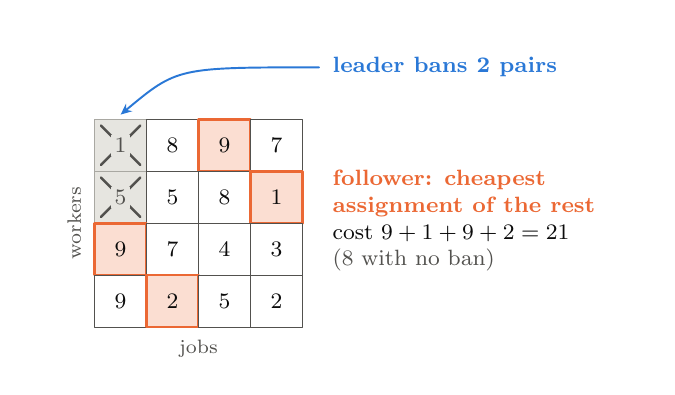
\begin{tikzpicture}
  % fixed page: 3.15 in x 1.75 in including the 2 pt border
  \useasboundingbox (0,0) rectangle (7.86,4.304);

  % the cost grid: banned (1,1), (2,1); assigned (1,3), (2,4), (3,1), (4,2)
  \cell{1}{1}{1}{1} \cell{1}{2}{8}{0} \cell{1}{3}{9}{2} \cell{1}{4}{7}{0}
  \cell{2}{1}{5}{1} \cell{2}{2}{5}{0} \cell{2}{3}{8}{0} \cell{2}{4}{1}{2}
  \cell{3}{1}{9}{2} \cell{3}{2}{7}{0} \cell{3}{3}{4}{0} \cell{3}{4}{3}{0}
  \cell{4}{1}{9}{0} \cell{4}{2}{2}{2} \cell{4}{3}{5}{0} \cell{4}{4}{2}{0}

  \node[small, text=ink2, anchor=north] at (\gx+2*\cs,\gy-0.04) {jobs};
  \node[small, text=ink2, rotate=90, anchor=south] at (\gx-0.05,\gy+2*\cs) {workers};

  % leader
  \node[anchor=west, align=left] at (3.75,3.80)
    {{\bfseries\color{leader}leader bans 2 pairs}};
  \draw[leader, line width=0.7pt, -{Stealth[length=4pt,width=3.5pt]}]
    (3.70,3.80) .. controls (1.9,3.80) .. (\gx+\cs/2,\gy+4*\cs+0.06);
  % follower
  \node[anchor=west, align=left] at (3.75,1.85)
    {{\bfseries\color{follower}follower: cheapest}\\
     {\bfseries\color{follower}assignment of the rest}\\
     cost $9+1+9+2 = 21$\\
     \textcolor{ink2}{(8 with no ban)}};
\end{tikzpicture}
\end{document}
